\chapter{Incertidumbre de la eficiencia corregida}\label{SecResulIncertidumbreEffMonteCarlo}
\begin{figure}
\centering
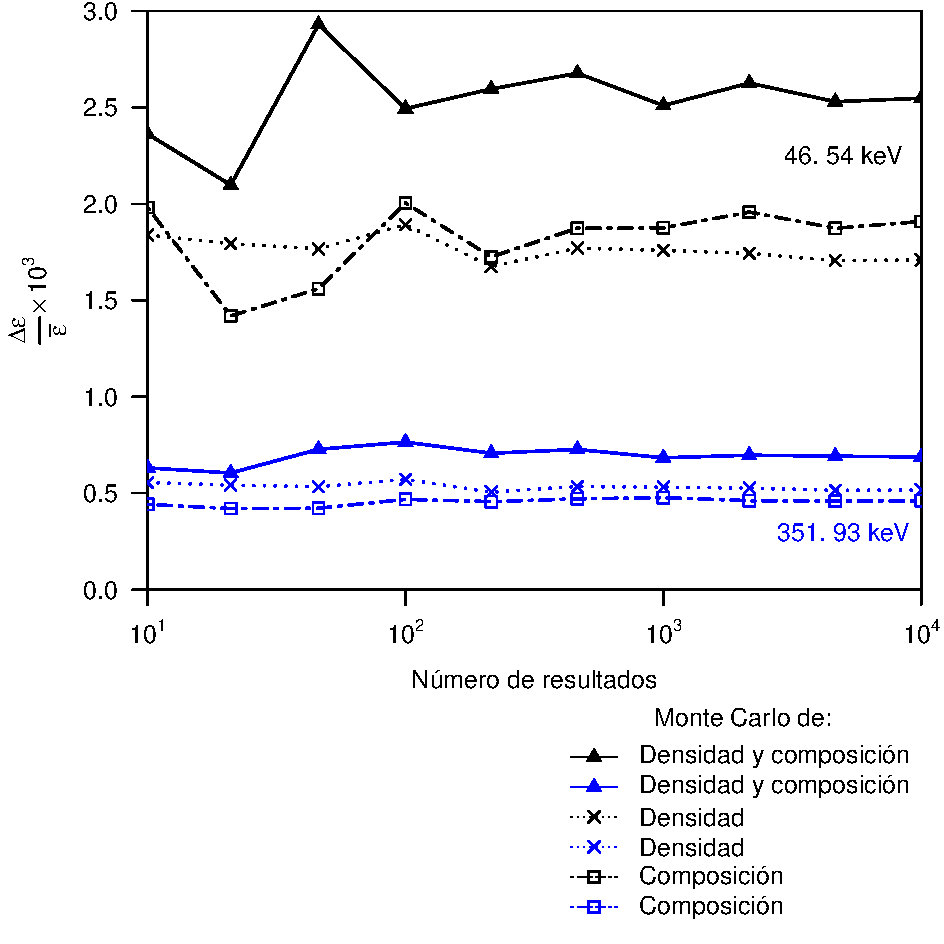
\includegraphics[width=\textwidth]{Imagenes/GOMRI-500_Eff_Point_Sec-21-75_cm.pdf}
\caption{Relación entre incertidumbre (sigma, $\Delta \epsilon$) y eficiencia promedio ($\bar{\epsilon}$) en función del número de simulaciones Monte Carlo variando el valor de la composición y / o densidad.}\label{Fig-MonteCarlo-Eficiencia}
\end{figure}
\lettrine{P}{}ara estimar la incertidumbre causada por la corrección de la eficiencia y densidad, se realizaron hasta 10$^{4}$ simulaciones con variabilidad de composición, densidad y ambas (Figura \ref{Fig-MonteCarlo-Eficiencia}). Se observó que las correcciones se estabilizan a partir de unas $10^3$ simulaciones. Las incertidumbres causadas por el proceso de corrección son muy pequeñas (Tabla \ref{Tabla-MonteCarlos-Effi}.), y fueron ignoradas en este trabajo. 
\\
\\
En este trabajo estudiamos la dependencia de la eficiencia corregida para las dos energías de interés (46.54 keV y 351.93 keV) entre 0.4 g cm$^{-3}$ y 1.5 g cm$^{-3}$, Figura \ref{Fig-EffDensidad2}. Si bien la eficiencia para el \PbCuatro\, es aproximadamente constante, para el \PbCero\, la eficiencia disminuye desde 0.66 hasta 0.53 en el intervalo de densidades analizadas.
\begin{table}
\centering
\caption{Variación de la eficiencia respecto a variaciones de la composición y/o densidad para $10^4$ repeticiones.}\label{Tabla-MonteCarlos-Effi}
\begin{tabular}{cccc}
\hline									
\rowcolor{Blue2}	Energía (keV)	&	Monte Carlo de:	&	$\bar{\epsilon} $	&	$\dfrac{\Delta \epsilon}{\bar{\epsilon}}\times 10^3 $	\\ 	\hline
\rowcolor{Blue1}	46.54	&	Composición	&	0.568255	&	1.9	\\ 	
\rowcolor{Blue1}		&	Densidad	&	0.568263	&	1.7	\\ 	
\rowcolor{Blue1}		&	Composición y densidad	&	0.568259	&	2.5	\\ 	\hline
\rowcolor{Blue1}	351.93	&	Composición	&	0.232834	&	0.5	\\ 	
\rowcolor{Blue1}		&	Densidad	&	0.232835	&	0.5	\\ 	
\rowcolor{Blue1}		&	Composición y densidad	&	0.232836	&	0.7	\\ 	\hline
\end{tabular}
\end{table}
\begin{figure}
\centering
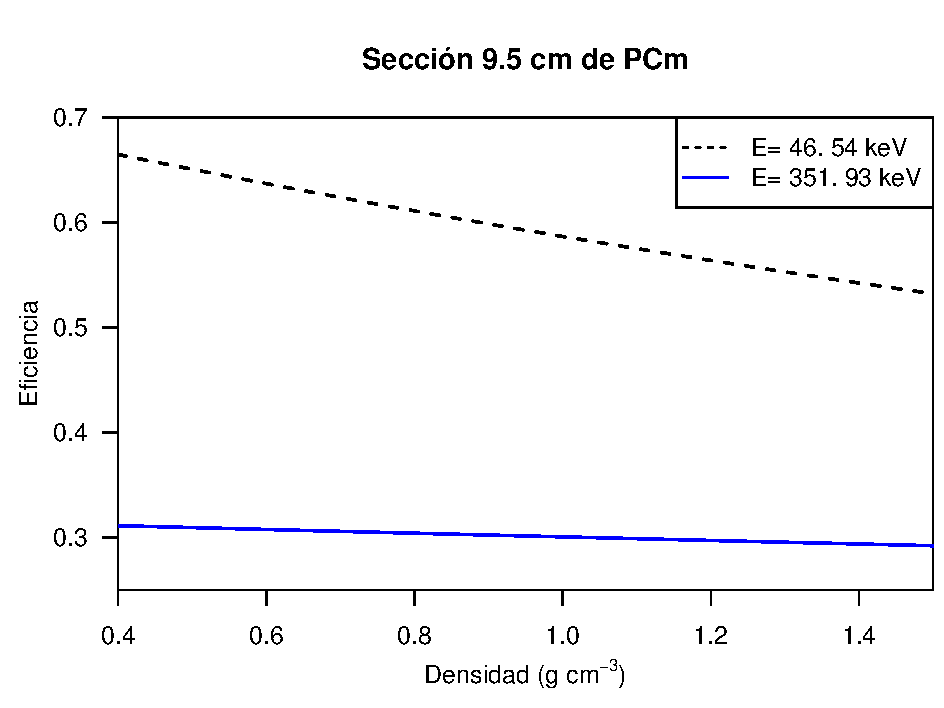
\includegraphics[width=0.9\textwidth]{Imagenes/Eficiencia-densidad.pdf}
\caption{Dependencia del valor de la eficiencia en función de la densidad para los valores de energías relacionados con \PbCero\, y \PbCuatro\, en la sección 9.5 cm del núcleo sedimentario PCm.}\label{Fig-EffDensidad2}
\end{figure}
